\chapter{DROP/SHIP} 
\label{sec:ships}
\lstset{style=6502Style}

The player deploys from a dropship. This ship is composed of 6 sprites tiled in 
two rows of three sprites each.

Individually these tiles are unremarkable - 
\raisebox{-0.2\totalheight}{
\includegraphics[height=0.4cm]{src/dropship_sprites/DROPSHIP_0.png}}
\raisebox{-0.2\totalheight}{
\includegraphics[height=0.4cm]{src/dropship_sprites/DROPSHIP_1.png}}
\raisebox{-0.2\totalheight}{
\includegraphics[height=0.4cm]{src/dropship_sprites/DROPSHIP_2.png}}
\raisebox{-0.2\totalheight}{
\includegraphics[height=0.4cm]{src/dropship_sprites/DROPSHIP_3.png}}
\raisebox{-0.2\totalheight}{
\includegraphics[height=0.4cm]{src/dropship_sprites/DROPSHIP_4.png}}
\raisebox{-0.2\totalheight}{
\includegraphics[height=0.4cm]{src/dropship_sprites/DROPSHIP_5.png}}
\raisebox{-0.2\totalheight}{
\includegraphics[height=0.4cm]{src/dropship_sprites/DROPSHIP_6.png}}
\raisebox{-0.2\totalheight}{
\includegraphics[height=0.4cm]{src/dropship_sprites/DROPSHIP_7.png}}
- and in the order that they appear it may not even be obvious that together they can form a whole.
But when properly combined they give us a chrome dropship from which the player's craft can emerge:

\begin{figure}[H]
    \centering
    \begin{adjustbox}{width=4cm,center}
      
\includegraphics{src/dropship_sprites/dropship.png}%
    \end{adjustbox}
\end{figure}

As with the manta craft itself, each of these sprites is built up from 63 bytes of data. On the following
page we can see the familiar diagrams from the rear of the dropship in detail. 
\clearpage

\begin{figure}[H]
    \centering
    \begin{adjustbox}{width=14cm,center}
      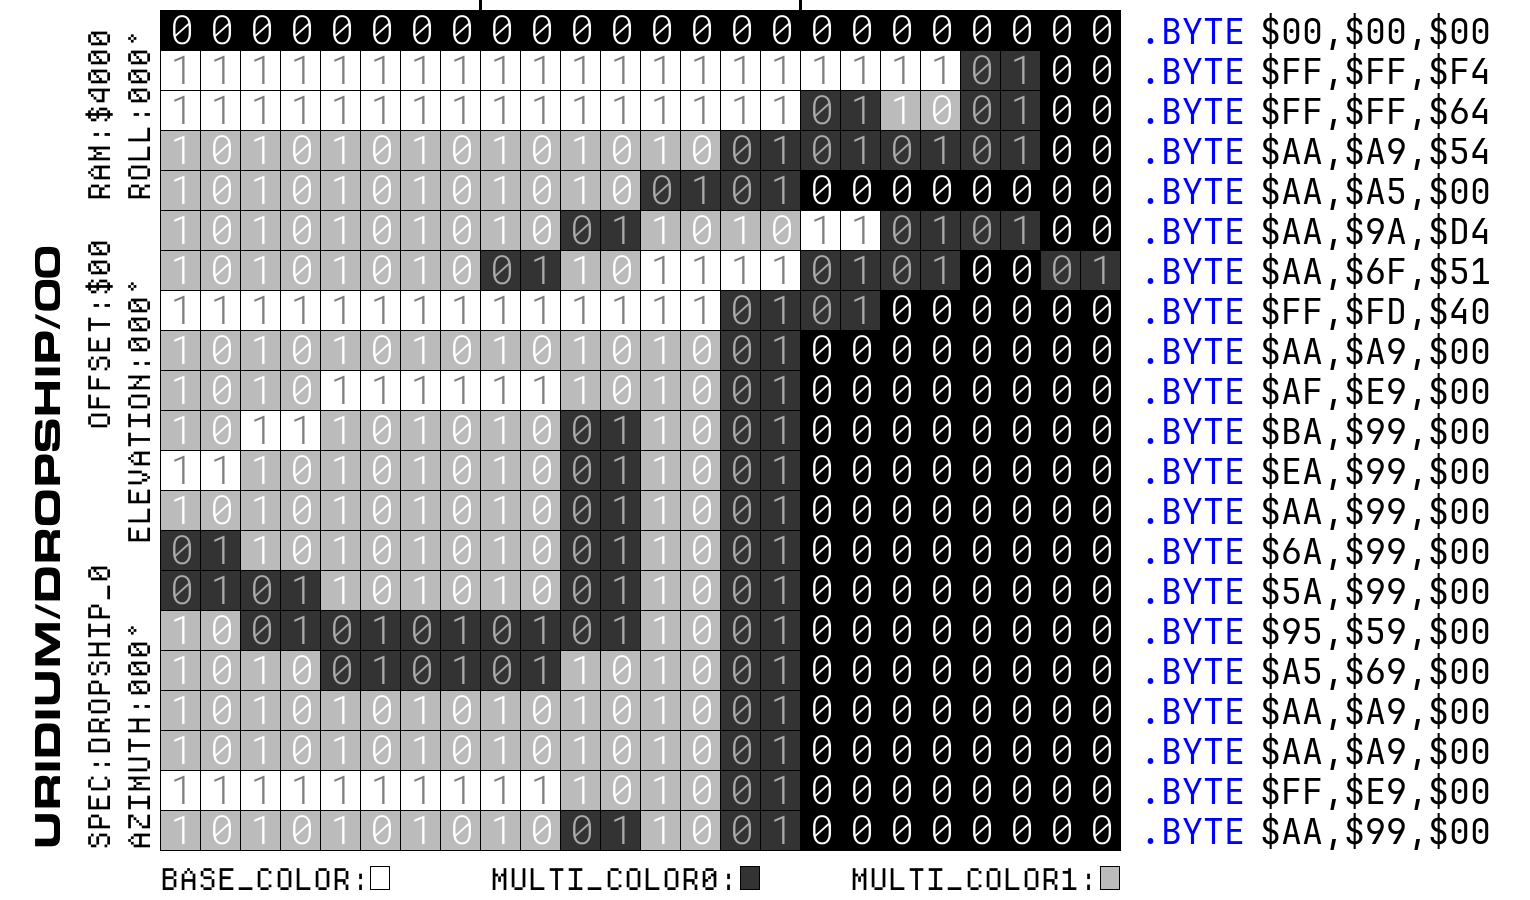
\includegraphics{src/dropship_diagrams_list/DROPSHIP_0.png}%
    \end{adjustbox}
\end{figure}
\begin{figure}[H]
    \centering
    \begin{adjustbox}{width=14cm,center}
      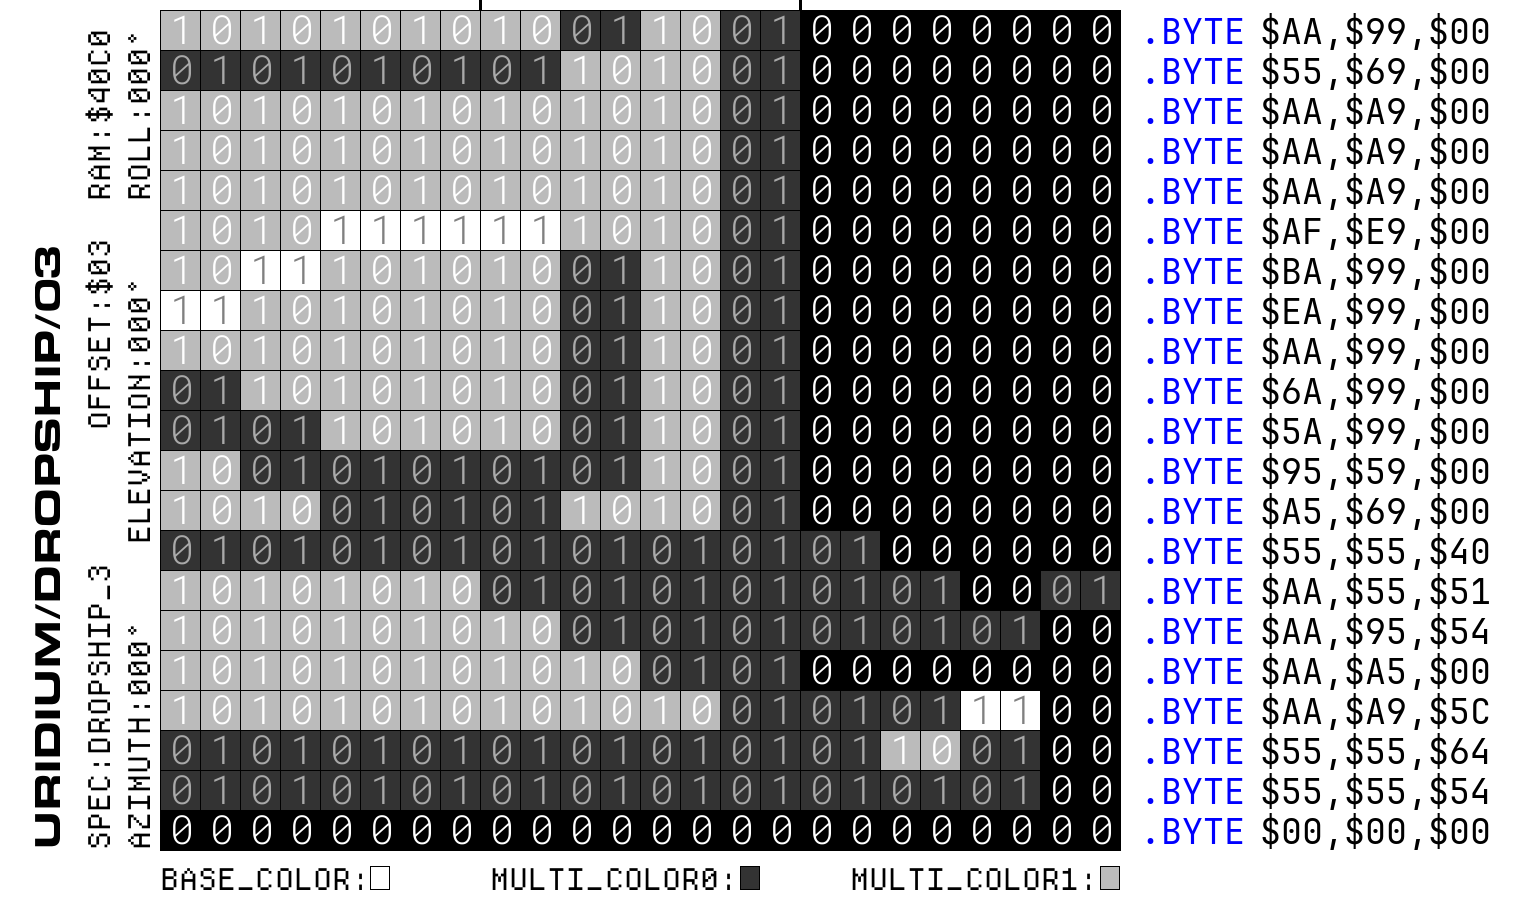
\includegraphics{src/dropship_diagrams_list/DROPSHIP_3.png}%
    \end{adjustbox}
\end{figure}

But if we zoom in slightly we can also see more about the order in which the sprites are composed.

\begin{figure}[H]
    \centering
    \begin{adjustbox}{width=14cm,center}
      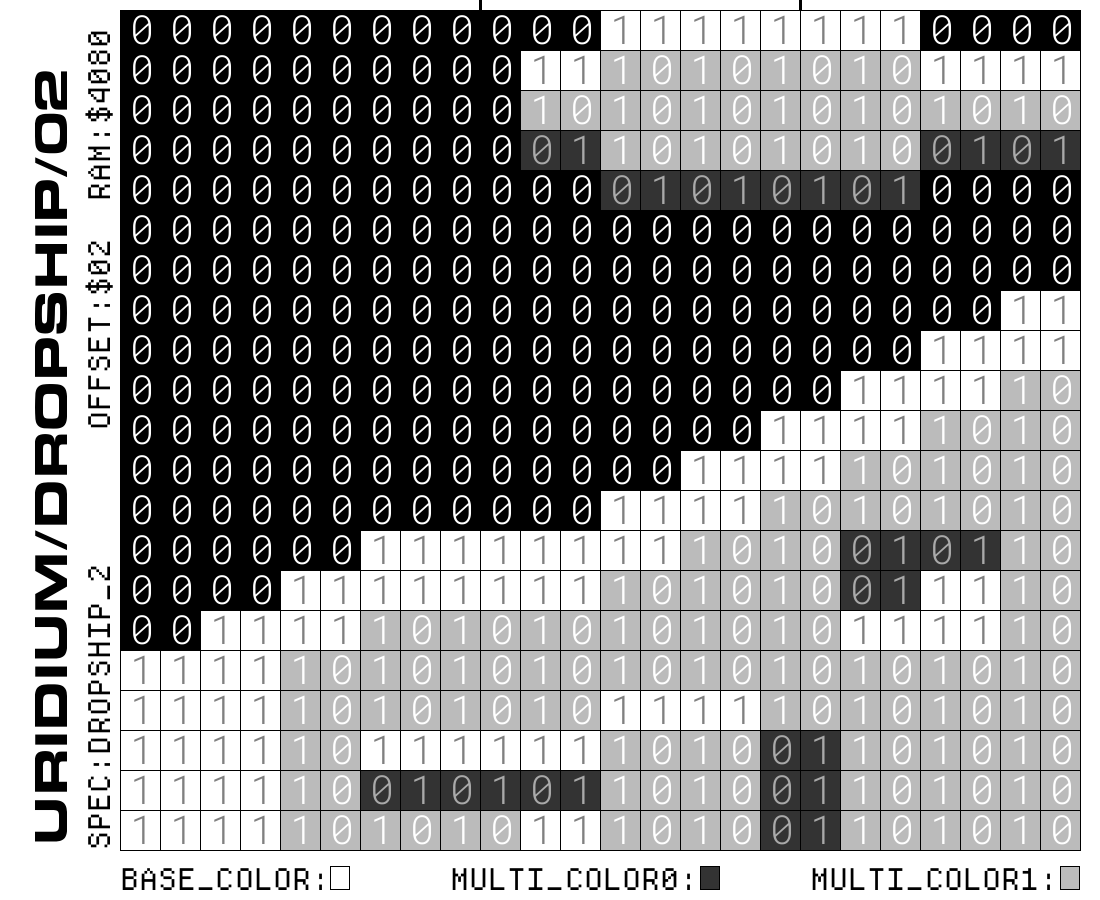
\includegraphics[width=7cm]{src/dropship_diagrams_list/DROPSHIP_BARE_2.png}%
			\hspace{-0.2cm}
      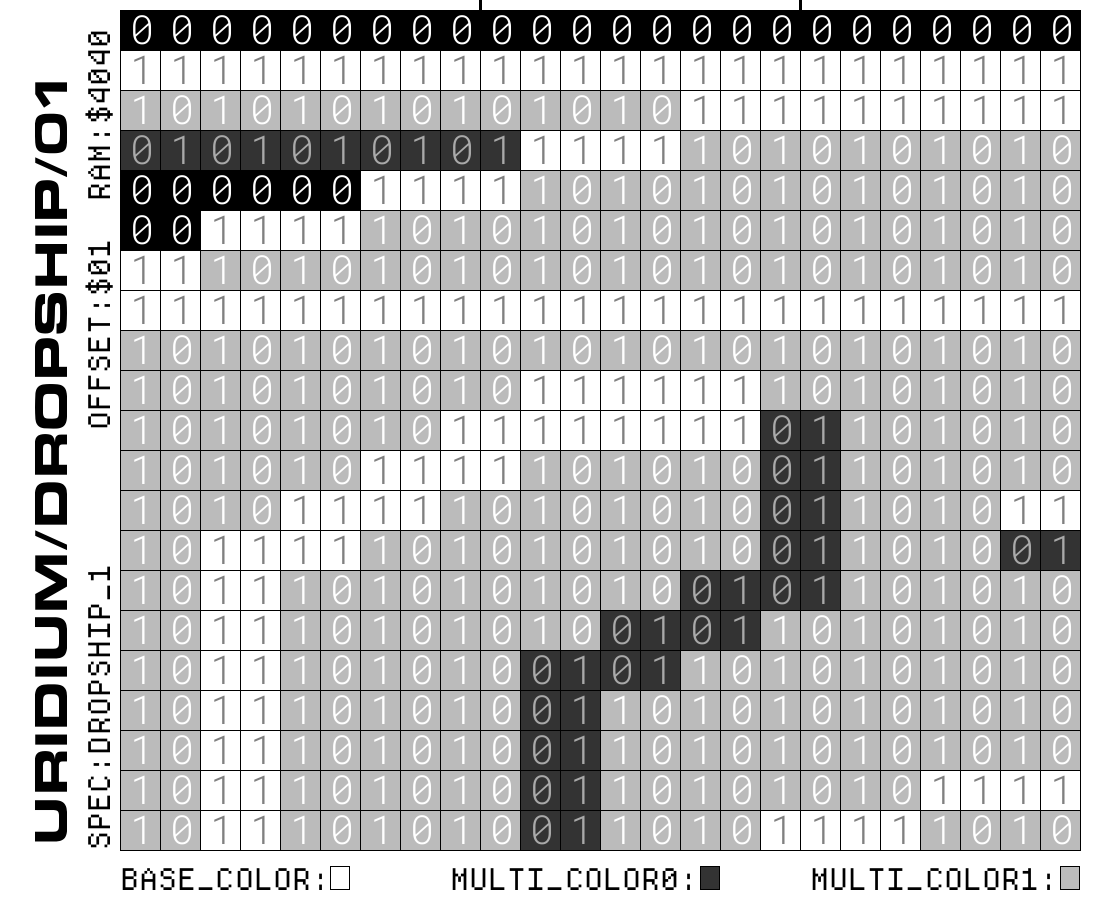
\includegraphics[width=7cm]{src/dropship_diagrams_list/DROPSHIP_BARE_1.png}%
			\hspace{-0.2cm}
      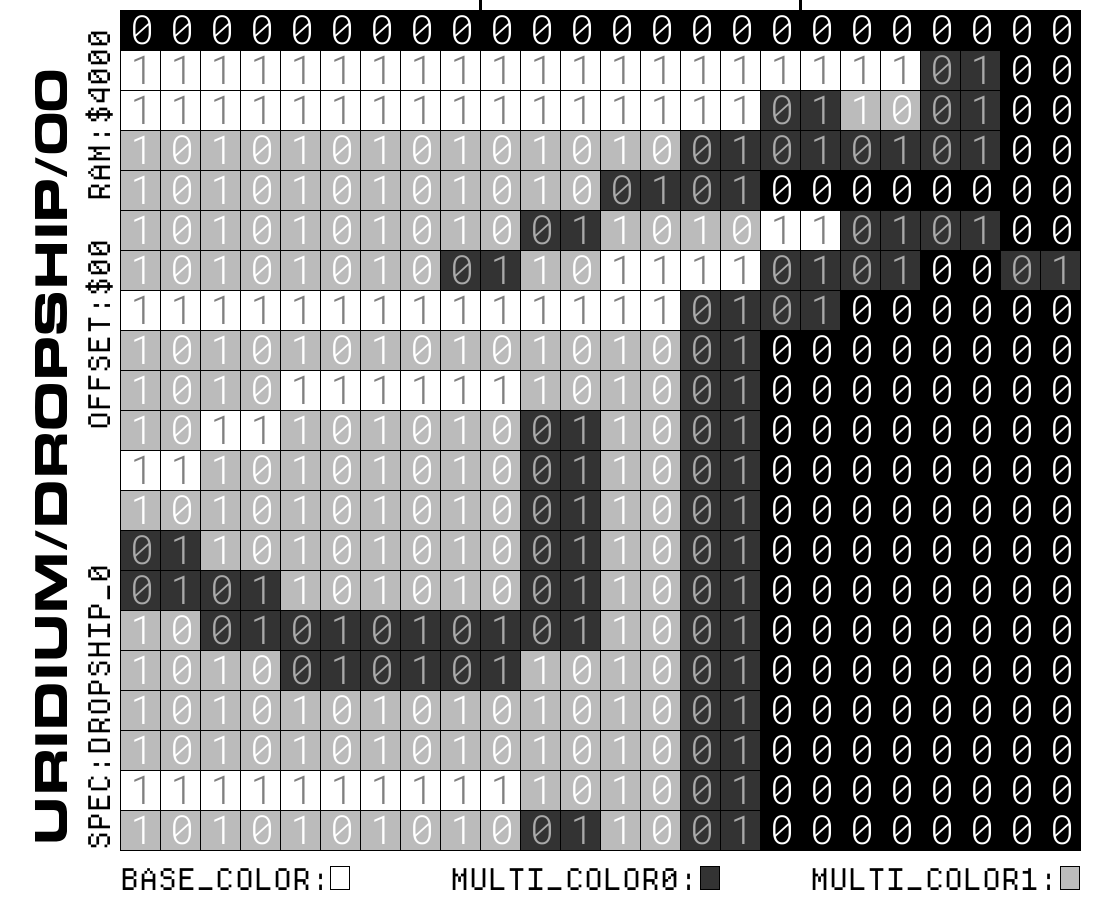
\includegraphics[width=7cm]{src/dropship_diagrams_list/DROPSHIP_BARE_0.png}%
    \end{adjustbox}
\end{figure}
\vspace{-1.05cm}
\begin{figure}[H]
    \centering
    \begin{adjustbox}{width=14cm,center}
      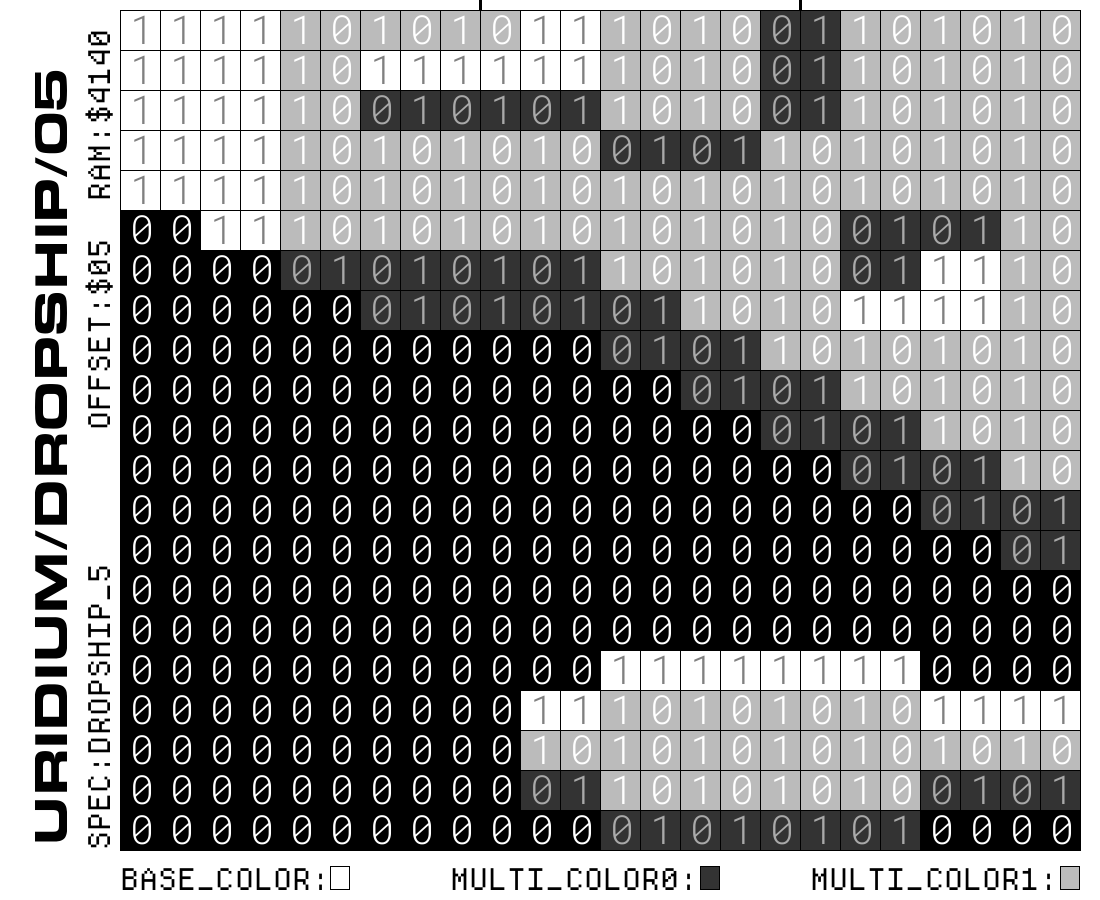
\includegraphics[width=7cm]{src/dropship_diagrams_list/DROPSHIP_BARE_5.png}%
			\hspace{-0.2cm}
      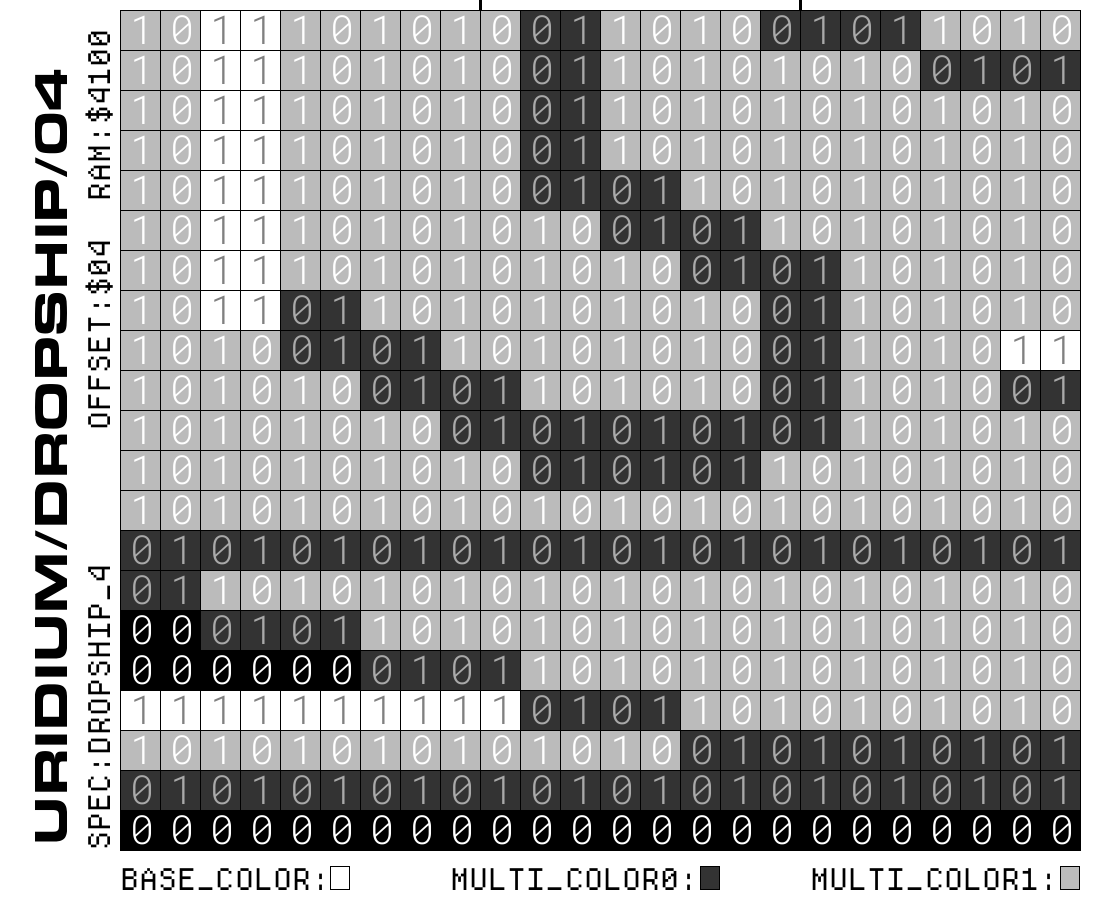
\includegraphics[width=7cm]{src/dropship_diagrams_list/DROPSHIP_BARE_4.png}%
			\hspace{-0.2cm}
      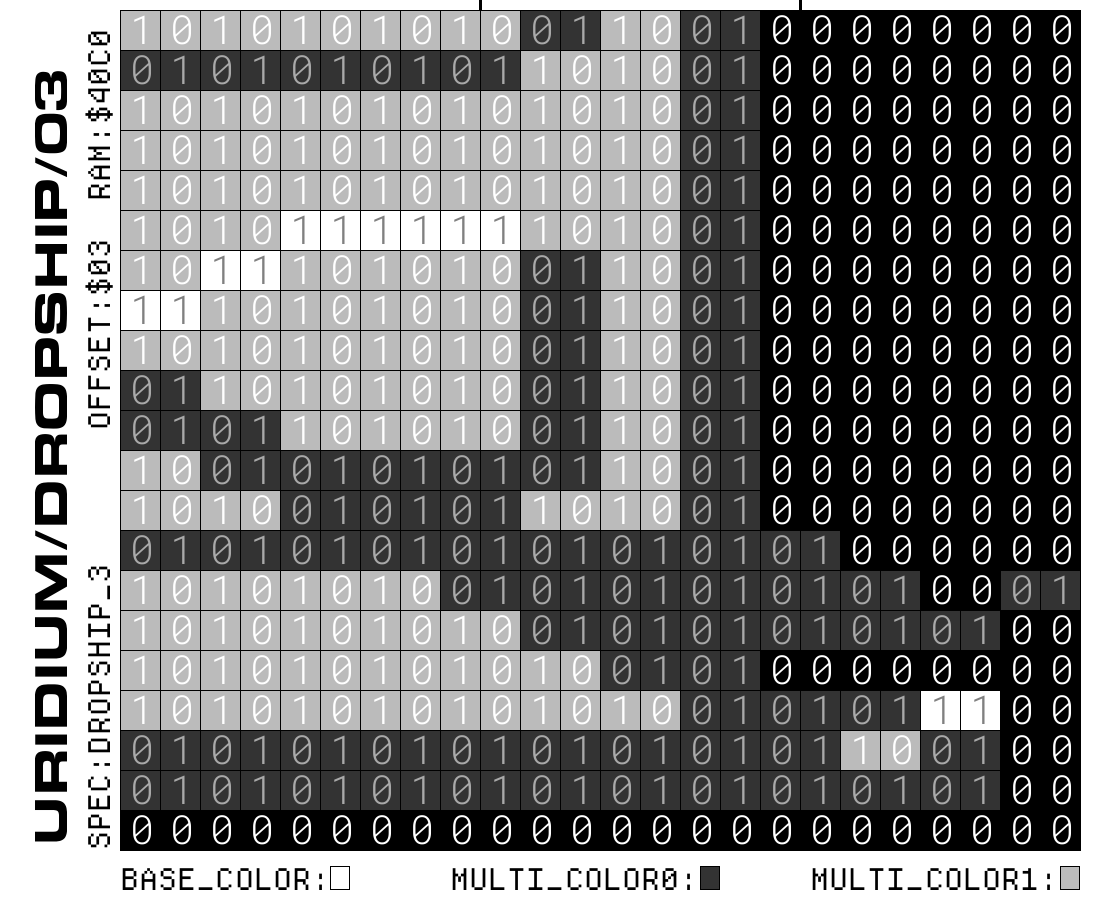
\includegraphics[width=7cm]{src/dropship_diagrams_list/DROPSHIP_BARE_3.png}%
    \end{adjustbox}
\end{figure}

We haven't included the landing bay at the rear of the craft in the montage above. This is because
there's a wrinkle we have to take account of in our addition of the sprite that depicts
the landing deck. This is evident when we see what happens we attempt it add it to the stern
of the dropship below: it's too small!

\begin{minipage}[c]{0.48\linewidth}
\vspace{-0.5cm}
\begin{figure}[H]
    \centering
    \begin{adjustbox}{width=7cm,left}
      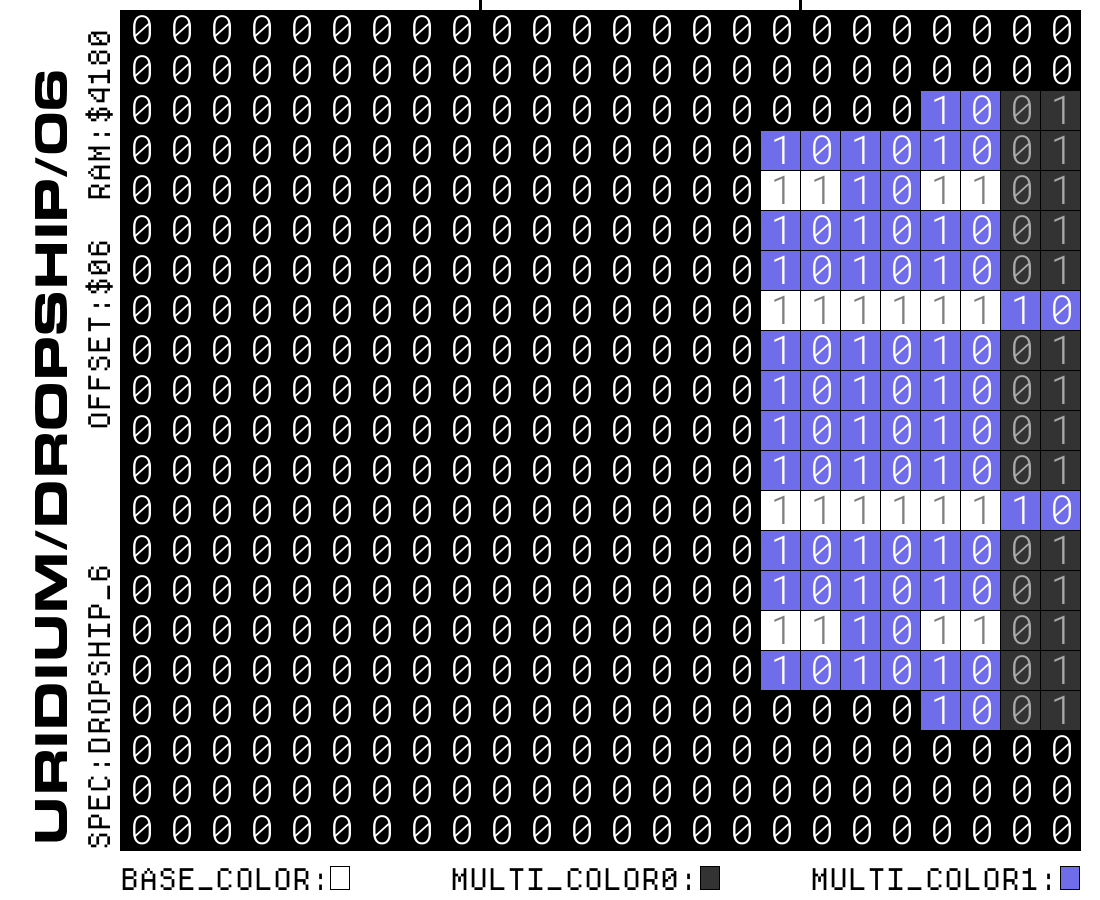
\includegraphics{src/dropship_diagrams_list/DROPSHIP_BARE_6.png}%
    \end{adjustbox}
\end{figure}
\end{minipage}
\hspace{0.6cm}
\begin{minipage}[c]{0.06\linewidth}
\begin{figure}[H]
    \centering
    
\begin{tikzpicture}[baseline={(current bounding box.south)}]
      \draw[->,line width=3pt] (0,0) to (1,0);
    \end{tikzpicture}
\end{figure}
\end{minipage}
\hspace{-0.3cm}
\begin{minipage}[c]{0.48\linewidth}
\vspace{-0.5cm}
\begin{figure}[H]
    \centering
    \begin{adjustbox}{width=4.2cm,center}
      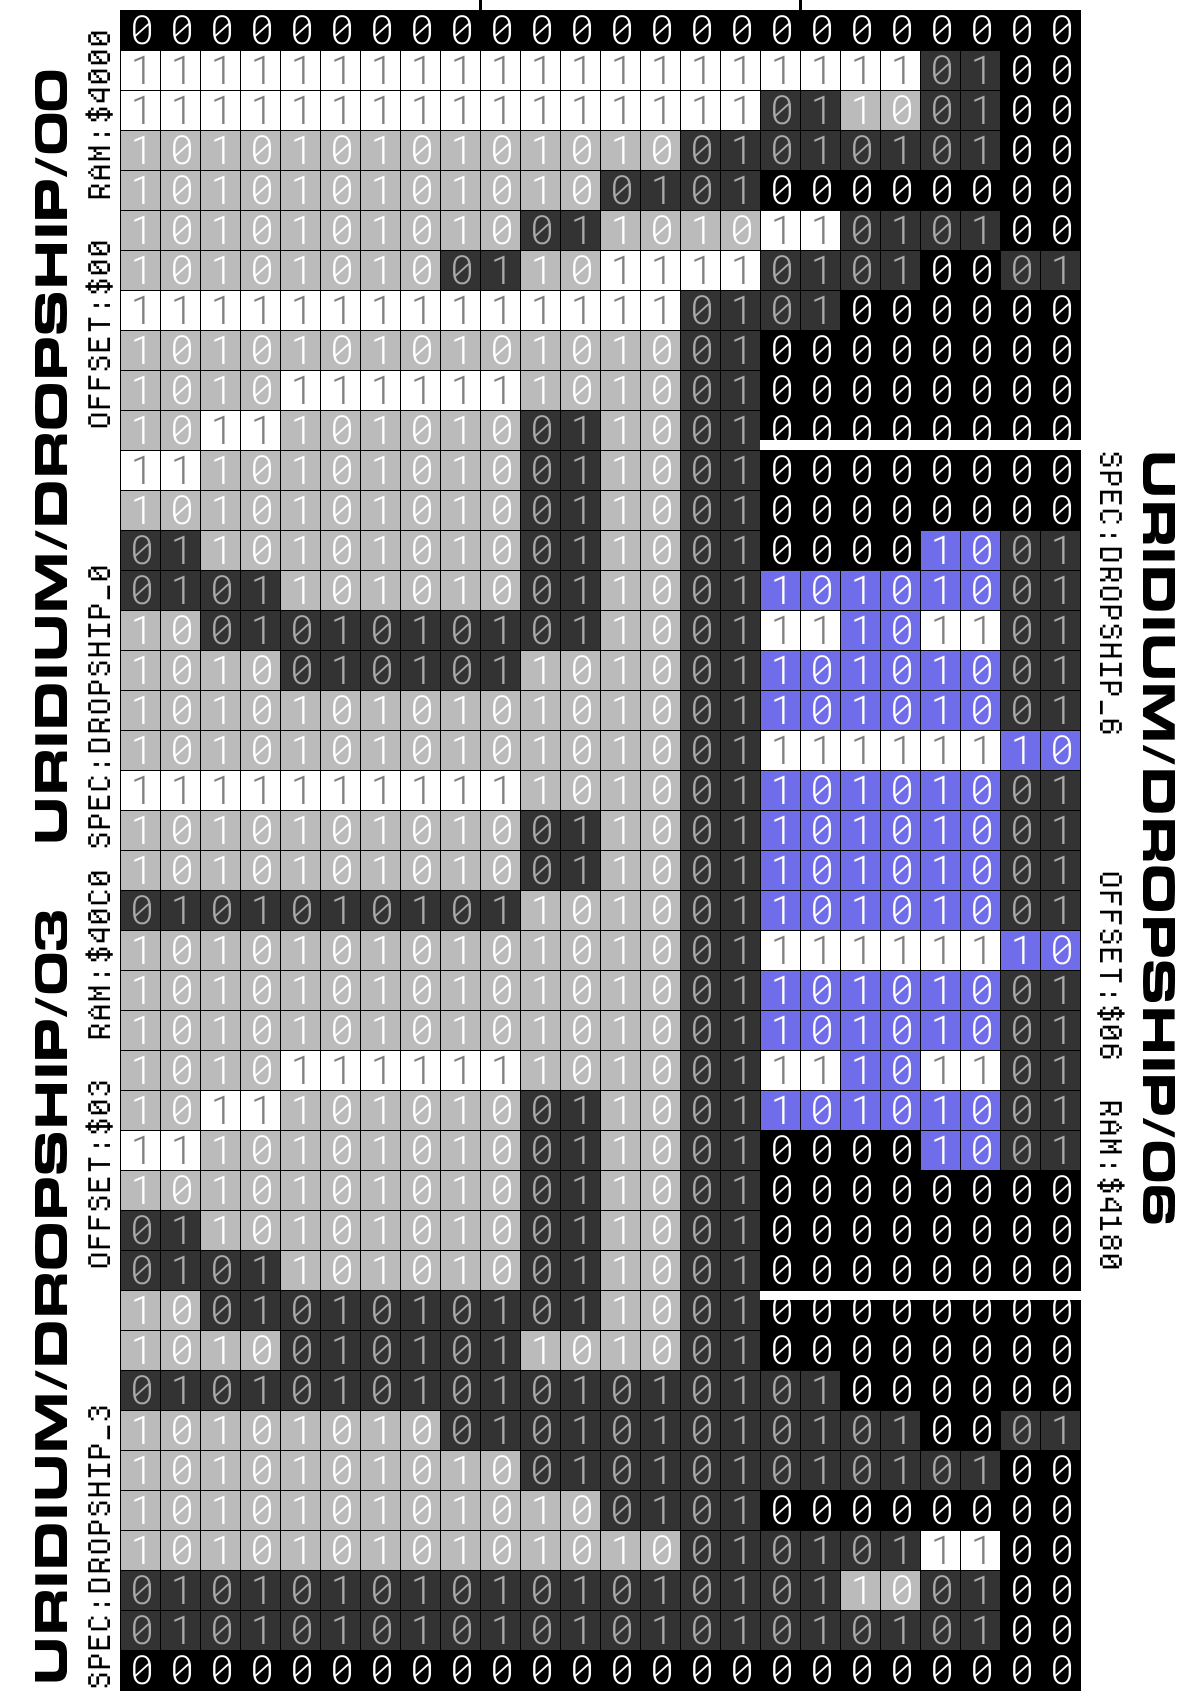
\includegraphics{src/dropship_diagrams_list/dropship_baydoor_unscaled.png}%
    \end{adjustbox}
\end{figure}
\end{minipage}

Why is this? Why doesn't it work like all the other sprites that make up the dropship? And what do
we have to do to make it work?
The answer is that we have to render the sprite in a slightly different way. We have to render each
row of bits twice. So our rendered sprite will be twice as high as a normal sprite, with 42 rows of pixels
rather than 21, and with each of the 21 rows in our data duplicated. How this works in practice is illustrated
below. And now the landing deck sprite fits neatly into place in the rear of the drop ship!

\begin{minipage}[c]{0.48\linewidth}
\vspace{-0.5cm}
\begin{figure}[H]
    \centering
    \begin{adjustbox}{width=6cm,left}
      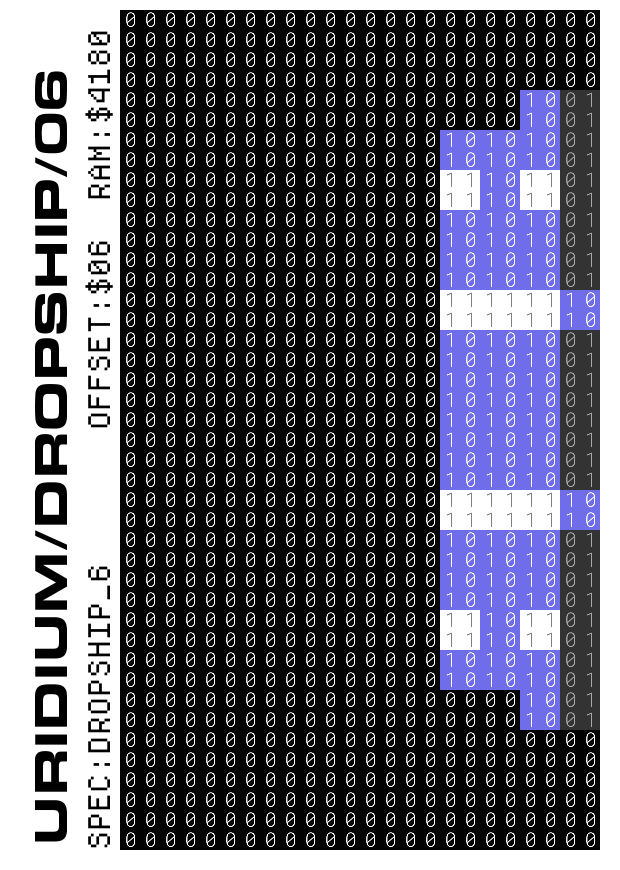
\includegraphics{src/dropship_diagrams_list/DROPSHIP_BARE_EXPANDED_6.png}%
    \end{adjustbox}
\end{figure}
\end{minipage}
\vspace{-0.1cm}
\hspace{-0.3cm}
\begin{minipage}[c]{0.06\linewidth}
\begin{figure}[H]
    \centering
    
\begin{tikzpicture}[baseline={(current bounding box.south)}]
      \draw[->,line width=3pt] (0,0) to (1,0);
    \end{tikzpicture}
\end{figure}
\end{minipage}
\vspace{-0.1cm}
\hspace{0.3cm}
\begin{minipage}[c]{0.48\linewidth}
\vspace{-0.5cm}
\begin{figure}[H]
    \centering
    \begin{adjustbox}{width=6cm,center}
      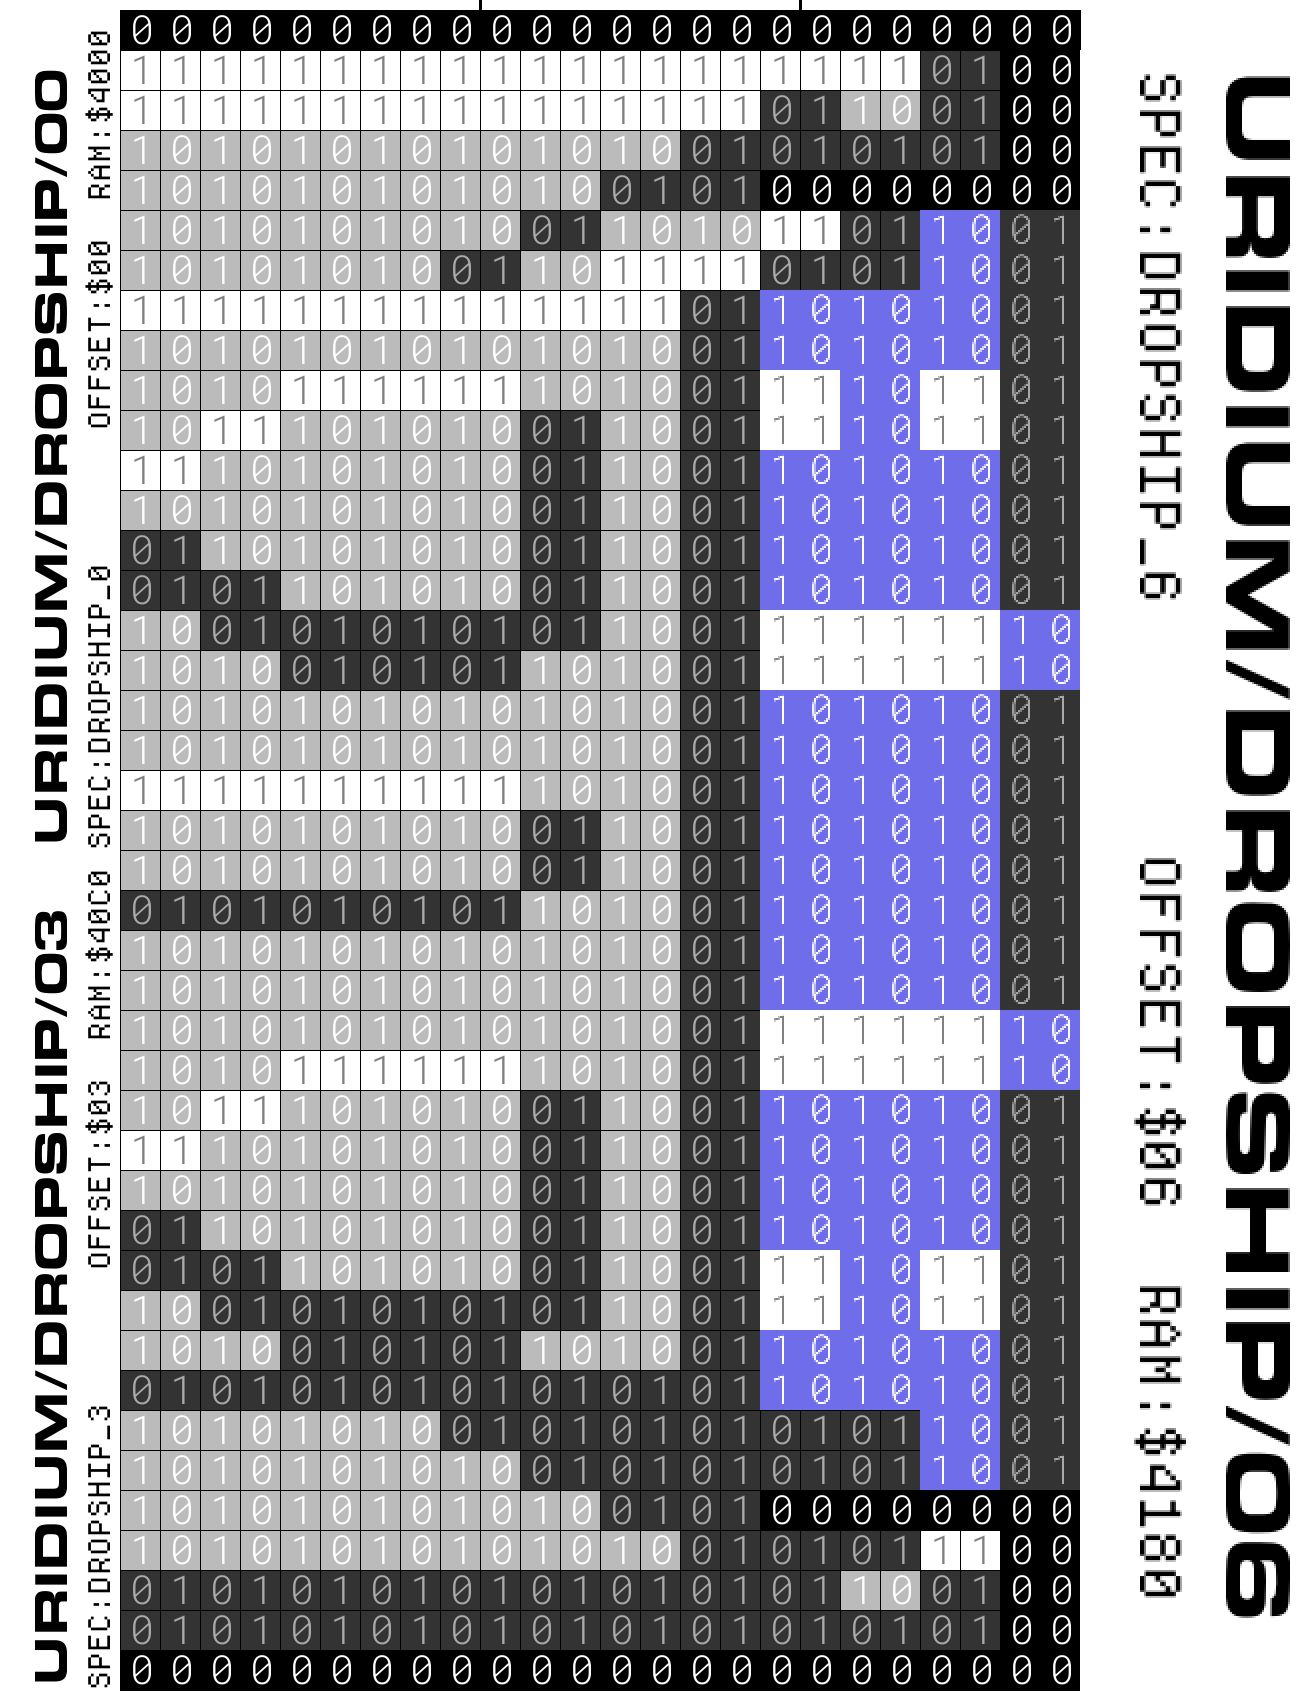
\includegraphics{src/dropship_diagrams_list/dropship_baydoor_scaled.png}%
    \end{adjustbox}
\end{figure}
\end{minipage}
\vspace{-0.1cm}

Now that we have an idea of how it has to work, let's briefly look at how the composition of the
drop ship is implemented in practice.
For each section that makes up the ship we will have an array of bytes detailing its position, its
color mode, and most importantly the actual sprite value to use. For example, this is what the section array
will look like for the section on the top right.

\begin{lstlisting}[escapechar=\%]
topRightSection
  .BYTE $00      ; Sprite's index.
  .BYTE $82      ; Sprite's X position.
  .BYTE $00      ; Sprite's supplemental X position.
  .BYTE $8D      ; Sprite's Y position.
  .BYTE $FF      ; Sprite Enabled/Disabled.
  .BYTE $00      ; Expand Vertical Off.
  .BYTE $00      ; Display Priority vs background.
  .BYTE $FF      ; Multi-Color Mode On.
  .BYTE $00      ; Expand Horizontal Off.
  .BYTE M_GRAY2  ; Sprite color (MULTI_COLOR_1).
  .BYTE %\raisebox{-0.2\totalheight}{
\includegraphics[height=0.4cm]{src/dropship_sprites/DROPSHIP_0.png}}%      ; Sprite Reference ($00).
\end{lstlisting}

And this is what the section array looks like for the landing deck. Notice that the byte that controls vertical
expansion is different from the value used for the \icode{topRightSection}. It is set to \icode{\$FF}, indicating
that each row of the sprite should be duplicated, doubling its vertical height as we require.

\begin{lstlisting}[escapechar=\%]
landingDeckSection
  .BYTE $07      ; Sprite's index.
  .BYTE $82      ; Sprite's X position.
  .BYTE $00      ; Sprite's supplemental X position.
  .BYTE $8E      ; Sprite's Y position.
  .BYTE $FF      ; Sprite Enabled.
  .BYTE $FF      ; Expand Vertical ON.
  .BYTE $00      ; Display Priority vs background.
  .BYTE $FF      ; Multi-Color Mode On.
  .BYTE $00      ; Expand Horizontal Off.
  .BYTE M_LTBLUE ; Sprite color (MULTI_COLOR_1).
  .BYTE%\raisebox{-0.2\totalheight}{
\includegraphics[height=0.4cm]{src/dropship_sprites/DROPSHIP_6.png}}%       ; Sprite Reference ($06).
\end{lstlisting}

With the details of each section defined in its own section array, we will now define an array that references each one. A 'list of lists' if you like.
\footnote{We actually define and use another as well: \icode{hiPtrsToDropShipSections}. This references the sections in the same order as \icode{loPtrsToDropShipSections}. We combine the entries in these arrays to get the two-byte address in memory where our section, such as \icode{topRightSection}, is located and read its data. This is what you see happening in \icode{DrawDropShip}.
}
Taken together, this array tells us the order
in which to place the sections. This order is important because when we draw one sprite after another each will obscure the one
before it, occluding any overlapping area.

\begin{lstlisting}[escapechar=\%]
loPtrsToDropShipSections
  .BYTE <topRightSection,     <topMiddleSection   ; %\raisebox{-0.2\totalheight}{
\includegraphics[height=0.31cm]{src/dropship_sprites/DROPSHIP_0.png}}% %\raisebox{-0.2\totalheight}{
\includegraphics[height=0.31cm]{src/dropship_sprites/DROPSHIP_1.png}}%
  .BYTE <topLeftSection,      <bottomRightSection ; %\raisebox{-0.2\totalheight}{
\includegraphics[height=0.31cm]{src/dropship_sprites/DROPSHIP_2.png}}% %\raisebox{-0.2\totalheight}{
\includegraphics[height=0.31cm]{src/dropship_sprites/DROPSHIP_3.png}}%
  .BYTE <bottomMiddleSection, <bottomLeftSection  ; %\raisebox{-0.2\totalheight}{
\includegraphics[height=0.31cm]{src/dropship_sprites/DROPSHIP_4.png}}% %\raisebox{-0.2\totalheight}{
\includegraphics[height=0.31cm]{src/dropship_sprites/DROPSHIP_5.png}}%
  .BYTE <bayDoorSection,  <landingDeckSection     ;  %\raisebox{-0.2\totalheight}{
\includegraphics[height=0.31cm]{src/dropship_sprites/DROPSHIP_7.png}}% %\raisebox{-0.2\totalheight}{
\includegraphics[height=0.31cm]{src/dropship_sprites/DROPSHIP_6.png}}%
\end{lstlisting}


Finally, we draw the drop ship using these data structures:
\begin{lstlisting}
  LDX #$07                       ; Start at the end of the section array.
DrawDropShip   
  LDA loPtrsToDropShipSections,X ; Get the X'th section from the array.
  STA sectionDataLoPtr           ; Store it.
  LDA hiPtrsToDropShipSections,X ; Get the X'th section from the array.
  STA sectionDataHiPtr           ; Store it.
  JSR LoadAndDisplaySectionData  ; Load the section and display it.
  DEX                            ; Move to the next section..
  BPL DrawDropShip               ; .. until we reach the first one.
\end{lstlisting}
In this snippet of code we iterate over the array of sections, starting at the end
of the array rather than the beginning, and draw each section. This means that the earlier sections will occlude the
later ones. Because the landing deck is at the end of the section array this means that any overlapping parts of the
deck will be occluded by the section above it, as we would expect if we were looking at in practice.

The illustration below shows how the craft is built up by the loop in \icode{DrawDropShip} above. We start with the landing deck and proceed
clockwise along the whole body of the dropship until it is complete.

\hspace{-1.5cm}
\raisebox{-0.2\totalheight}{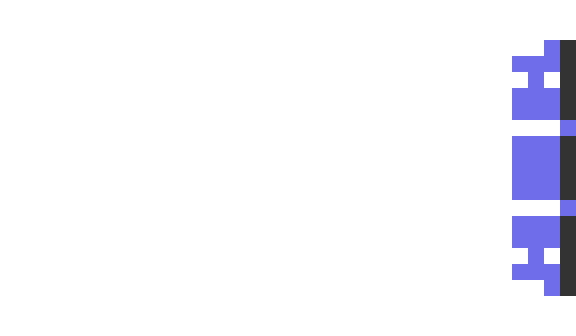
\includegraphics[height=1.2cm]{src/dropship_sprites/dropship_gradual_0.png}}
\hspace{-1.0cm}
\raisebox{-0.2\totalheight}{
\includegraphics[height=1.2cm]{src/dropship_sprites/dropship_gradual_1.png}}
\hspace{-0.3cm}
\raisebox{-0.2\totalheight}{
\includegraphics[height=1.2cm]{src/dropship_sprites/dropship_gradual_2.png}}
\hspace{0.1cm}
\raisebox{-0.2\totalheight}{
\includegraphics[height=1.2cm]{src/dropship_sprites/dropship_gradual_3.png}}
\hspace{0.1cm}
\raisebox{-0.2\totalheight}{
\includegraphics[height=1.2cm]{src/dropship_sprites/dropship_gradual_4.png}}
\hspace{0.1cm}
\raisebox{-0.2\totalheight}{
\includegraphics[height=1.2cm]{src/dropship_sprites/dropship_gradual_5.png}}
\hspace{0.1cm}
\raisebox{-0.2\totalheight}{
\includegraphics[height=1.2cm]{src/dropship_sprites/dropship_gradual_6.png}}




